%\documentclass{beamer} % presentation class
\documentclass[handout]{beamer} % for printout class
%\documentclass[trans]{beamer} % for iPad notes class

% for handouts
\usepackage{pgfpages}
\pgfpagesdeclarelayout{6 on 1}
{
  \edef\pgfpageoptionheight{\the\paperwidth} % landscaped by default
  \edef\pgfpageoptionwidth{\the\paperheight}
  \def\pgfpageoptionborder{0pt}
  \def\pgfpageoptionfirstshipout{1}
}
{
  \pgfpagesphysicalpageoptions
  {%
    logical pages=6,%
    physical height=\pgfpageoptionheight,%
    physical width=\pgfpageoptionwidth,%
    current logical shipout=\pgfpageoptionfirstshipout%
  }
  \ifdim\paperheight>\paperwidth\relax
    % put side-by-side
    \pgfpageslogicalpageoptions{1}
    {%
      border shrink=\pgfpageoptionborder,%
      resized width=.5\pgfphysicalwidth,%
      resized height=\pgfphysicalheight,%
      center=\pgfpoint{.1667\pgfphysicalwidth}{.25\pgfphysicalheight}%
    }%
    \pgfpageslogicalpageoptions{3}
    {%
      border shrink=\pgfpageoptionborder,%
      resized width=.5\pgfphysicalwidth,%
      resized height=\pgfphysicalheight,%
      center=\pgfpoint{.5\pgfphysicalwidth}{.25\pgfphysicalheight}%
    }%
    \pgfpageslogicalpageoptions{5}
    {%
      border shrink=\pgfpageoptionborder,%
      resized width=.5\pgfphysicalwidth,%
      resized height=\pgfphysicalheight,%
      center=\pgfpoint{.8333\pgfphysicalwidth}{.25\pgfphysicalheight}%
    }%
    \pgfpageslogicalpageoptions{2}
    {%
      border shrink=\pgfpageoptionborder,%
      resized width=.5\pgfphysicalwidth,%
      resized height=\pgfphysicalheight,%
      center=\pgfpoint{.1667\pgfphysicalwidth}{.75\pgfphysicalheight}%
    }%
    \pgfpageslogicalpageoptions{4}
    {%
      border shrink=\pgfpageoptionborder,%
      resized width=.5\pgfphysicalwidth,%
      resized height=\pgfphysicalheight,%
      center=\pgfpoint{.5\pgfphysicalwidth}{.75\pgfphysicalheight}%
    }%
    \pgfpageslogicalpageoptions{6}
    {%
      border shrink=\pgfpageoptionborder,%
      resized width=.5\pgfphysicalwidth,%
      resized height=\pgfphysicalheight,%
      center=\pgfpoint{.8333\pgfphysicalwidth}{.75\pgfphysicalheight}%
    }%
  \else
    % stack on top of one another
    \pgfpageslogicalpageoptions{1}
    {%
      border shrink=\pgfpageoptionborder,%
      resized width=0.5\pgfphysicalwidth,%
      resized height=\pgfphysicalheight,%
      center=\pgfpoint{.25\pgfphysicalwidth}{.8333\pgfphysicalheight}%
    }%
    \pgfpageslogicalpageoptions{3}
    {%
      border shrink=\pgfpageoptionborder,%
      resized width=0.5\pgfphysicalwidth,%
      resized height=\pgfphysicalheight,%
      center=\pgfpoint{.25\pgfphysicalwidth}{.5\pgfphysicalheight}%
    }%
    \pgfpageslogicalpageoptions{5}
    {%
      border shrink=\pgfpageoptionborder,%
      resized width=0.5\pgfphysicalwidth,%
      resized height=\pgfphysicalheight,%
      center=\pgfpoint{.25\pgfphysicalwidth}{.1667\pgfphysicalheight}%
    }%
    \pgfpageslogicalpageoptions{2}
    {%
      border shrink=\pgfpageoptionborder,%
      resized width=0.5\pgfphysicalwidth,%
      resized height=\pgfphysicalheight,%
      center=\pgfpoint{.75\pgfphysicalwidth}{.8333\pgfphysicalheight}%
    }%
    \pgfpageslogicalpageoptions{4}
    {%
      border shrink=\pgfpageoptionborder,%
      resized width=0.5\pgfphysicalwidth,%
      resized height=\pgfphysicalheight,%
      center=\pgfpoint{.75\pgfphysicalwidth}{.5\pgfphysicalheight}%
    }%
    \pgfpageslogicalpageoptions{6}
    {%
      border shrink=\pgfpageoptionborder,%
      resized width=0.5\pgfphysicalwidth,%
      resized height=\pgfphysicalheight,%
      center=\pgfpoint{.75\pgfphysicalwidth}{.1667\pgfphysicalheight}%
    }%
  \fi
}

%\pgfpagesuselayout{6 on 1}[letterpaper,landscape,border shrink=5mm]

% The theme to use
\mode<presentation>
{
  \useoutertheme[footline=empty, subsection=false]{miniframes}
	\usecolortheme{sandystonebeachoceandiver}
  \setbeamercovered{transparent}
	\setbeamertemplate{navigation symbols}{}
}

\mode<handout>{
    \pgfpagesuselayout{6 on 1}[letterpaper,border shrink=0mm]
    \pgfpageslogicalpageoptions{1}{border code=\pgfusepath{stroke}}
    \pgfpageslogicalpageoptions{2}{border code=\pgfusepath{stroke}}
    \pgfpageslogicalpageoptions{3}{border code=\pgfusepath{stroke}}
    \pgfpageslogicalpageoptions{4}{border code=\pgfusepath{stroke}}
    \pgfpageslogicalpageoptions{5}{border code=\pgfusepath{stroke}}
    \pgfpageslogicalpageoptions{6}{border code=\pgfusepath{stroke}}
		\setbeameroption{show notes}
}

\mode<trans>{
	\setbeameroption{show only notes}
}


\usepackage{attrib} % for quoting bible verses with attribution
\usepackage{xstring} % more complex strings
\usepackage{graphicx} % graphics inclusion
\usepackage[english]{babel}
\usepackage[latin1]{inputenc}
\usepackage{times}
\usepackage[T1]{fontenc}
\usepackage{remreset}% tiny package containing just the 


\includeonlylecture{03} % including on a lect


%% Get the points on the presentation without subsections
\makeatletter
\@removefromreset{subsection}{section}
\makeatother
\setcounter{subsection}{1}

%% macros for removing slide dots on demand
\makeatletter
\let\beamer@writeslidentry@miniframeson=\beamer@writeslidentry
\def\beamer@writeslidentry@miniframesoff{%
  \expandafter\beamer@ifempty\expandafter{\beamer@framestartpage}{}% does not happen normally
  {%else
    % removed \addtocontents commands
    \clearpage\beamer@notesactions%
  }
}
\newcommand*{\miniframeson}{\let\beamer@writeslidentry=\beamer@writeslidentry@miniframeson}
\newcommand*{\miniframesoff}{\let\beamer@writeslidentry=\beamer@writeslidentry@miniframesoff}
\makeatother

%%%%%%%%%%%%%%
% Custom macros and environments
\newenvironment{goals}
{
\newcommand{\goal}{\item[--]}
\begin{frame}[fragile,environment=goals]
\frametitle{Goals}
\begin{itemize}	
}
{\end{itemize}
\end{frame}
}

\newcommand{\versehighlight}[2]{
\expandarg
\StrSubstitute{#2}{#1}{\alert{#1}}
}

\newcommand{\keyverse}{
31 Behold, the days are coming, declares the Lord, when I will make a new covenant with the house of Israel and the house of Judah, 32 not like the covenant that I made with their fathers on the day when I took them by the hand to bring them out of the land of Egypt, my covenant that they broke, though I was their husband, declares the Lord. 33 For this is the covenant that I will make with the house of Israel after those days, declares the Lord: I will put my law within them, and I will write it on their hearts. And I will be their God, and they shall be my people. 34 And no longer shall each one teach his neighbor and each his brother, saying, `Know the Lord,' for they shall all know me, from the least of them to the greatest, declares the Lord. For I will forgive their iniquity, and I will remember their sin no more.}

\newcommand{\keyversehiglight}[1]{
\versehighlight{#1}{\keyverse}
}

%%%%%%%%%%%%%%
\title[] % (optional, use only with long paper titles)
{``For They Shall All Know Me''}

\subtitle
{Developing a New Covenant Relationship with God} % (optional)

%\author[Author, Another] % (optional, use only with lots of authors)
%{F.~Author\inst{1} \and S.~Another\inst{2}}
% - Use the \inst{?} command only if the authors have different
%   affiliation.

%\institute[Universities of Somewhere and Elsewhere] % (optional, but mostly needed)
%{
%  \inst{1}%
  %Department of Computer Science\\
  %University of Somewhere
  %\and
  %Department of Theoretical Philosophy\\
  %\inst{2}%
  %University of Elsewhere}
%% - Use the \inst command only if there are several affiliations.
%% - Keep it simple, no one is interested in your street address.

\date[Sun. AM] % (optional)
{Spring 2016 / Sunday AM Bible Study}

\subject{Sunday morning classes Walnut Street Church of Christ}

\pgfdeclareimage[height=3cm]{touchOfGod}{figures/creation_of_adam.png}
\titlegraphic{\pgfuseimage{touchOfGod}\\{\tiny \emph{Workbook}~~Print goo.gl/iSmU50~~Phone goo.gl/KCzzWU~~Tablet goo.gl/FgxaKp}}

%	 This is only inserted into the PDF information catalog. Can be left
% out. 



% If you have a file called "university-logo-filename.xxx", where xxx
% is a graphic format that can be processed by latex or pdflatex,
% resp., then you can add a logo as follows:

%\pgfdeclareimage[height=0.3cm]{logo}{figures/walnutstcoc_logo_bw.png}
%\logo{{\tiny Walnut Street Church of Christ} \pgfuseimage{logo}}



% Delete this, if you do not want the table of contents to pop up at
% the beginning of each subsection:
%\AtBeginSubsection[]
%{
  %\begin{frame}<beamer>{Outline}
    %\tableofcontents[currentsection,currentsubsection]
  %\end{frame}
%}

% When having one big beamer document for the entire course you can customize the output for each class.
\AtBeginLecture{
\miniframesoff
\frame{\Large Lesson~\insertlecture}
\miniframeson
%\begin{frame}{Outline}
%  \tableofcontents
%  % You might wish to add the option [pausesections]
%\end{frame}
}

% If you wish to uncover everything in a step-wise fashion, uncomment
% the following command: 
%\beamerdefaultoverlayspecification{<+->}


\begin{document}

\miniframesoff
\begin{frame}[plain]
  \titlepage
\end{frame}
\miniframeson

\lecture{Introduction}{01-Introduction}
% - Exactly two or three sections (other than the summary).
% - At *most* three subsections per section.
% - Talk about 30s to 2min per frame. So there should be between about
%   15 and 30 frames, all told.

\section{Introduction}

\begin{goals}
\goal Become familiar with the class theme, key passage, and class objectives.
\goal Understand how each subsequent lesson fits into the class objectives.
\goal Do an initial evaluation of how relationship-focused your religion is.
\end{goals}

\begin{frame}
\begin{quote}
31 Behold, the days are coming, declares the Lord, when I will make a new covenant with the house of Israel and the house of Judah, 32 not like the covenant that I made with their fathers on the day when I took them by the hand to bring them out of the land of Egypt, my covenant that they broke, though I was their husband, declares the Lord. 33 For this is the covenant that I will make with the house of Israel after those days, declares the Lord: I will put my law within them, and I will write it on their hearts. And I will be their God, and they shall be my people. \attrib{Jeremiah 31:31-33}
\end{quote}
\end{frame}

%\begin{discussion}
%\dsubsec{Introduction}{900-905}{5}
%
%This lesson is about who God is.
%
%\bvs{Genesis}{(17:1-8)} God's first covenant with Abraham says that he will be his God.
%
%\dsubsec{Who is God?}{905-915}{10}
%
	%\bvs{Psalms}{(8:1-9)} It's amazing that God is is mindful of us.
%
%\dsubsec{How we come to know about God}{915-925}{10}
%
	%\bvs{Ecclesiastes}{(3:11)} Eternity in the heart of man
%
  %\bvs{Hebrews}{(1:1-2)} Fathers by the prophets, today His son
	%
	%By extension His Word.
%
%\dsubsec{What does that mean for me?}{925-940}{15}
%
	%\bvs{Luke}{(4:1-13)} Having a God gives you an anchor. 
	%
	%\bvs{Luke}{(14:25-27)} Love God and you will live.
%
%\dsubsec{Review}{940-945}{5}
%\end{discussion}

%\begin{frame}{Class Theme}{Subtitles are optional.}
  %% - A title should summarize the slide in an understandable fashion
  %%   for anyone how does not follow everything on the slide itself.
%
  %\begin{itemize}
  %\item
    %Use \texttt{itemize} a lot.
  %\item
    %Use very short sentences or short phrases.
  %\end{itemize}
%\end{frame}
%\begin{frame}{Lesson Motivation}{Subtitles are optional.}
  %% - A title should summarize the slide in an understandable fashion
  %%   for anyone how does not follow everything on the slide itself.
%
  %\begin{itemize}
  %\item
    %Use \texttt{itemize} a lot.
  %\item
    %Use very short sentences or short phrases.
  %\end{itemize}
%\end{frame}
%\begin{frame}{Lesson Objectives}{Subtitles are optional.}
  %% - A title should summarize the slide in an understandable fashion
  %%   for anyone how does not follow everything on the slide itself.
%
  %\begin{itemize}
  %\item
    %Use \texttt{itemize} a lot.
  %\item
    %Use very short sentences or short phrases.
  %\end{itemize}
%\end{frame}
%\section{Point1}
%\section{Point2}
%\section{Point3}
%\subsection[Objectives]{Theme}
%\subsection[Short First Subsection Name]{First Subsection Name}
%
%\begin{frame}{Make Titles Informative. Use Uppercase Letters.}{Subtitles are optional.}
  %% - A title should summarize the slide in an understandable fashion
  %%   for anyone how does not follow everything on the slide itself.
%
  %\begin{itemize}
  %\item
    %Use \texttt{itemize} a lot.
  %\item
    %Use very short sentences or short phrases.
  %\end{itemize}
%\end{frame}
%
%\begin{frame}{Make Titles Informative.}
%
  %You can create overlays\dots
  %\begin{itemize}
  %\item using the \texttt{pause} command:
    %\begin{itemize}
    %\item
      %First item.
      %\pause
    %\item    
      %Second item.
    %\end{itemize}
  %\item
    %using overlay specifications:
    %\begin{itemize}
    %\item<3->
      %First item.
    %\item<4->
      %Second item.
    %\end{itemize}
  %\item
    %using the general \texttt{uncover} command:
    %\begin{itemize}
      %\uncover<5->{\item
        %First item.}
      %\uncover<6->{\item
        %Second item.}
    %\end{itemize}
  %\end{itemize}
%\end{frame}
%
%
%\subsection{Second Subsection}
%
%\begin{frame}{Make Titles Informative.}
%\end{frame}
%
%\begin{frame}{Make Titles Informative.}
%\end{frame}
%
%
%
%\section*{Summary}
%
%\begin{frame}{Summary}
%
  %% Keep the summary *very short*.
  %\begin{itemize}
  %\item
    %The \alert{first main message} of your talk in one or two lines.
  %\item
    %The \alert{second main message} of your talk in one or two lines.
  %\item
    %Perhaps a \alert{third message}, but not more than that.
  %\end{itemize}
  %
  %% The following outlook is optional.
  %\vskip0pt plus.5fill
  %\begin{itemize}
  %\item
    %Outlook
    %\begin{itemize}
    %\item
      %Something you haven't solved.
    %\item
      %Something else you haven't solved.
    %\end{itemize}
  %\end{itemize}
%\end{frame}


\lecture{2. I will be their God}{02}

\section*{Introduction}

\begin{frame}
\frametitle{Texas is my state}
	\begin{center}
	
\includegraphics[width=.9\textwidth]{figures/texas.jpg}
	\end{center}
\note{09:30}
\note[item]{I, like most Texans, am proud where I come from.}
\note[item]{Texans are taught that their state is simply better than any other state (or country).}
\note[item]{God wants us to think that way about Him -- that He is simply better.}
\note[item]{He is the only one that deserves our loyalty.}
\note[item]{He wants His team to be the only team we play for.}
\end{frame}

\begin{frame}
\frametitle{God wants a relationship with people}
\framesubtitle{Jeremiah 31:31-34}
	\keyversehiglight{I will be their God}
	\note{09:32}
	\note[item]{In our class we're trying to establish, from the Bible, the idea that God 
wants a relationship with people.}
	\note[item]{We're using Jeremiah 31:31-34 as a means of focusing that study.}
	\note[item]{Jeremiah 31:31-34 is one of the most important passages in the Bible, because it provides a connection between the old covenant and the new covenant, and talks about the close, special relationship that God's chosen people have with Him.  Under the old covenant, those people were the Israelites.  Under the New Covenant, those special people are all Christians.}
	\note[item]{\emph{Read it}}
	\note[item]{Today we'll be talking about how God wants to be the only God in our lives.}
\end{frame}

\begin{goals}
\goal Consider who God is, and consider how He is similar and different from man.
\goal Explore the different ways God has revealed himself to man.
\goal Think about ways to improve my perspective on who God is.

\note{09:33}
\note[item]{Examine why God is worthy of our loyalty.}
\note[item]{Examine how we learn about God's greatness.}
\note[item]{Considering how we can increase our devotion to God.}
\end{goals}

\section{I will be your God}

\begin{frame}
\frametitle{I will be your God}
\framesubtitle{Gen 17:1-8}
\begin{columns}[T]
	\begin{column}{0.4\textwidth}
		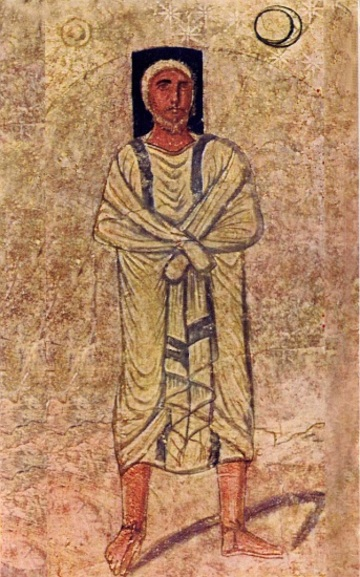
\includegraphics[height=0.8\textheight]{figures/abrahamDuraEuropos.jpg}
	\end{column}
	\begin{column}{0.6\textwidth}
		``And I will give you and to your offspring after you the land of your sojournings, all the land of Canaan, for an everlasting possession, and \\\alert{I will be their God}.'' -- Genesis 17:8
	\end{column}
\end{columns}

\note{09:35}
\note[item]{God recounts his 3-fold promise to Abraham: land, nation, seed (if you count ``kings shall come from you'')}.
\note[item]{Part or all of these promises are repeated at various times in Abraham's life (Gen 12, 13, 15, 17, 22)}
\note[item]{The first occurrence of the phrase `I will be their God' is in God's promise to Abraham.}
\note[item]{Fresco pictured here is one of the earliest depictions of a Bible narrative.  It depicts Abraham and God's promises to Him.  It is from the Dura-Europos synagogue 244 AD  70\% of the city has been destroyed during the Syrian civil war.}
\note[item]{When does God mean when he says `I will be their God'? \emph{Abraham had many `gods' to choose from, but God wanted Abraham to love only Him.}}
\note[item]{vs.1-2 Because God is mighty, he had to put a condition on His covenant with Abraham -- be blameless.}
\end{frame}

\begin{frame}
\frametitle{`I will be their God' through the Bible}
\begin{columns}[T]
	\begin{column}{0.45\textwidth}
		`I will be their God'\\{\footnotesize Gen. 17:8, Jer. 24:7, Jer. 31:33\\Jer. 32:36, Jer. 32:38, Ez. 11:20\\Ez. 37:15, Ez. 37:23, Ez. 37:27\\Zech. 8:8, 2 Cor. 6:16, Heb. 8:10}\\~\\
		`I will be your God'\\{\footnotesize Ex. 6:7, Jer. 7:23, Jer. 11:4\\Jer. 30:2, Ez. 36:28}\\~\\
	\end{column}
	\begin{column}{0.55\textwidth}
			`the Lord your God'\\ 
			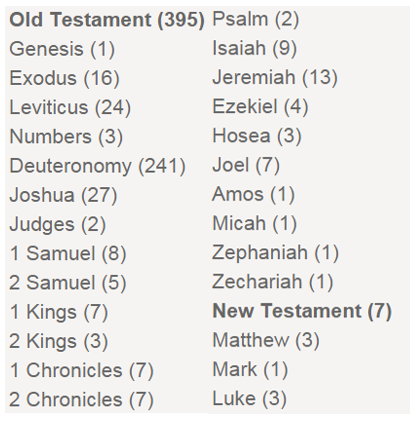
\includegraphics[width=1\columnwidth]{figures/theLordYourGodTwoColumn.png}
	\end{column}
\end{columns}

\note{09:38}
\note[item]{Last week, `your God', given to the Israelites as part of the Law of Moses (Ex. 6:1-9, Lev. 22:31-33).}
\note[item]{Clearly God thinks it's important that we view Him as the only God.}
\note[item]{It's not just that His people accept Him as the `true' God.  But as `their' God}
\end{frame}

\section{Who is God?}

\begin{frame}
\frametitle{God is majestic}
\framesubtitle{Psalm 8}
\begin{center}
	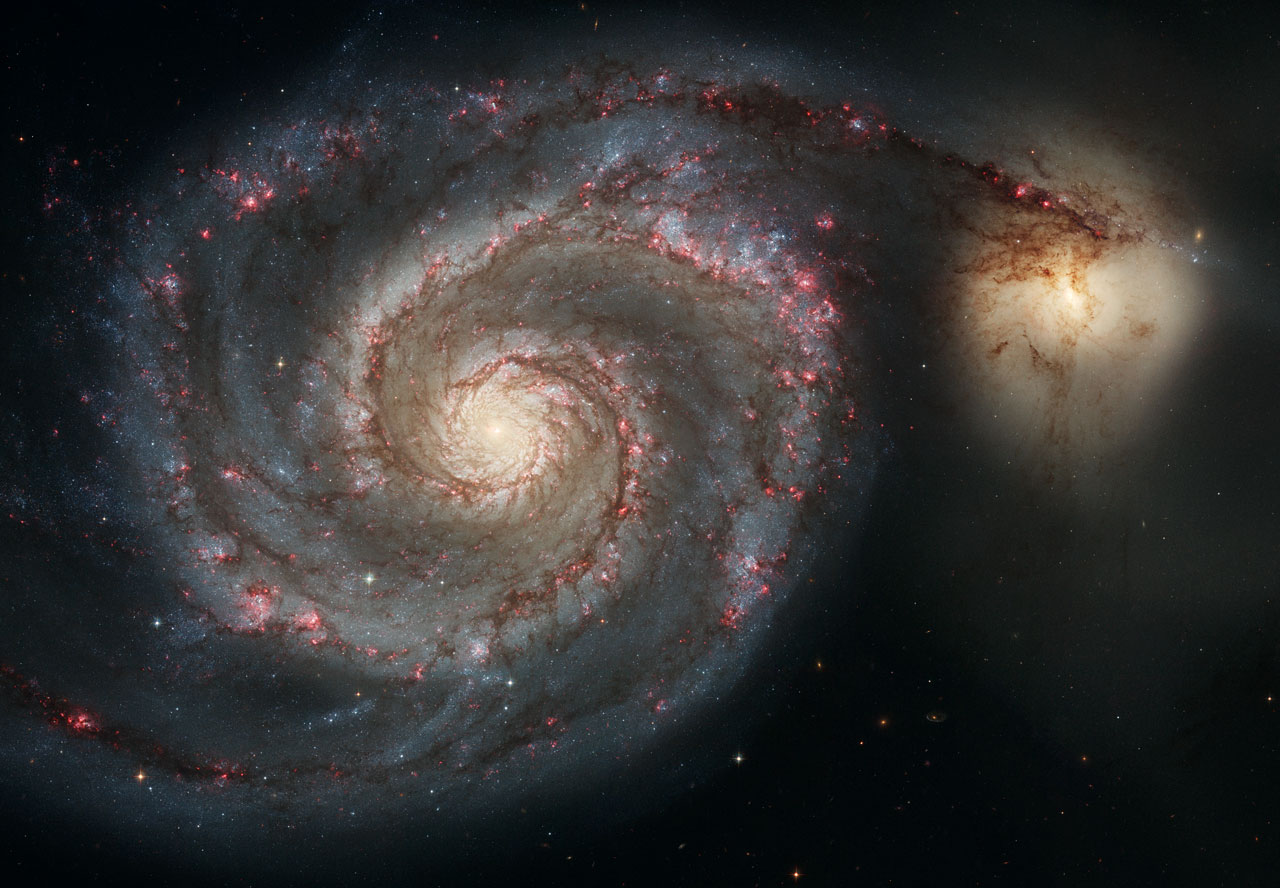
\includegraphics[width=0.85\textwidth]{figures/galaxy.jpg}\\
	{\footnotesize The Whirlpool galaxy as seen from the Hubble Space Telescope}
\end{center}

\note{09:40}
\note[item]{The Whirlpool galaxy is 60,000 LY across.  You can see it clearly with your own telescope.  Right below the handle of the big dipper.}
\note[item]{I'm small compared to God.}
\end{frame}

\begin{frame}
\frametitle{Man is not the source of God's greatness}
\framesubtitle{Psalm 8}
Out of the mouth of babes and sucklings hast thou perfected praise, because of thine enemies; that thou mightest put down the enemy and avenger.\hfill--Psalm 8:2 (LXX)\\~\\
15 But when the chief priests and the scribes saw the wonderful things that he did, and the children crying out in the temple, ``Hosanna to the Son of David!'' they were indignant, 16 and they said to him, ``Do you hear what these are saying?'' And Jesus said to them, ``Yes; have you never read,
\begin{quote}
`Out of the mouth of infants and nursing babies you have prepared praise'?
\end{quote}\\
\hfill-- Matt. 21:15-16 (ESV)
\normalsize

\note{09:41}
\note[item]{In context, Psalm 8:2 may refer to Israel, who followed the true God, being small and the surrounding nations being `great'.}
\note[item]{Jesus quotes Psalm 8:2 to remind the chief priests and scribes that they are not the source of His approval.}
\note[item]{It's important to remember that God is great, whether or not man accepts it.}
\end{frame}

\begin{frame}
\frametitle{God loves man and has blessed him.}
\framesubtitle{Psalm 8}
\begin{center}
	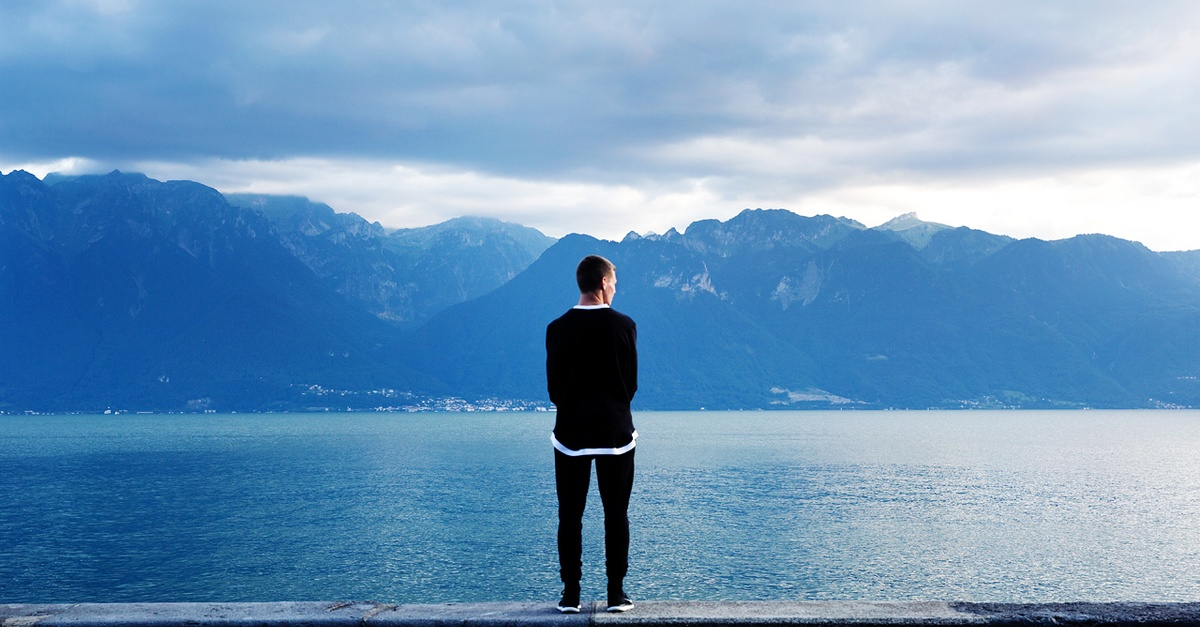
\includegraphics[width=\textwidth]{figures/manLandscape.jpg}\\
	``The worst moment for the atheist is when he is really thankful and has nobody to thank.''
\end{center}

\note{09:45}
\note[item]{Man is not powerful like God is.}
\note[item]{Yet, He has made us special compared to all other creation}
\note[item]{Man is special and loved even when he rejects God.}
\note[item]{Quote is possibly attributed to Dante Gabriel Rossetti, a painter poet from the mid-19th century}
\end{frame}

\section{How we come to know about God}

\begin{frame}
\frametitle{Eternity is set in the heart of man}
\framesubtitle{Ecclesiastes 3:11}
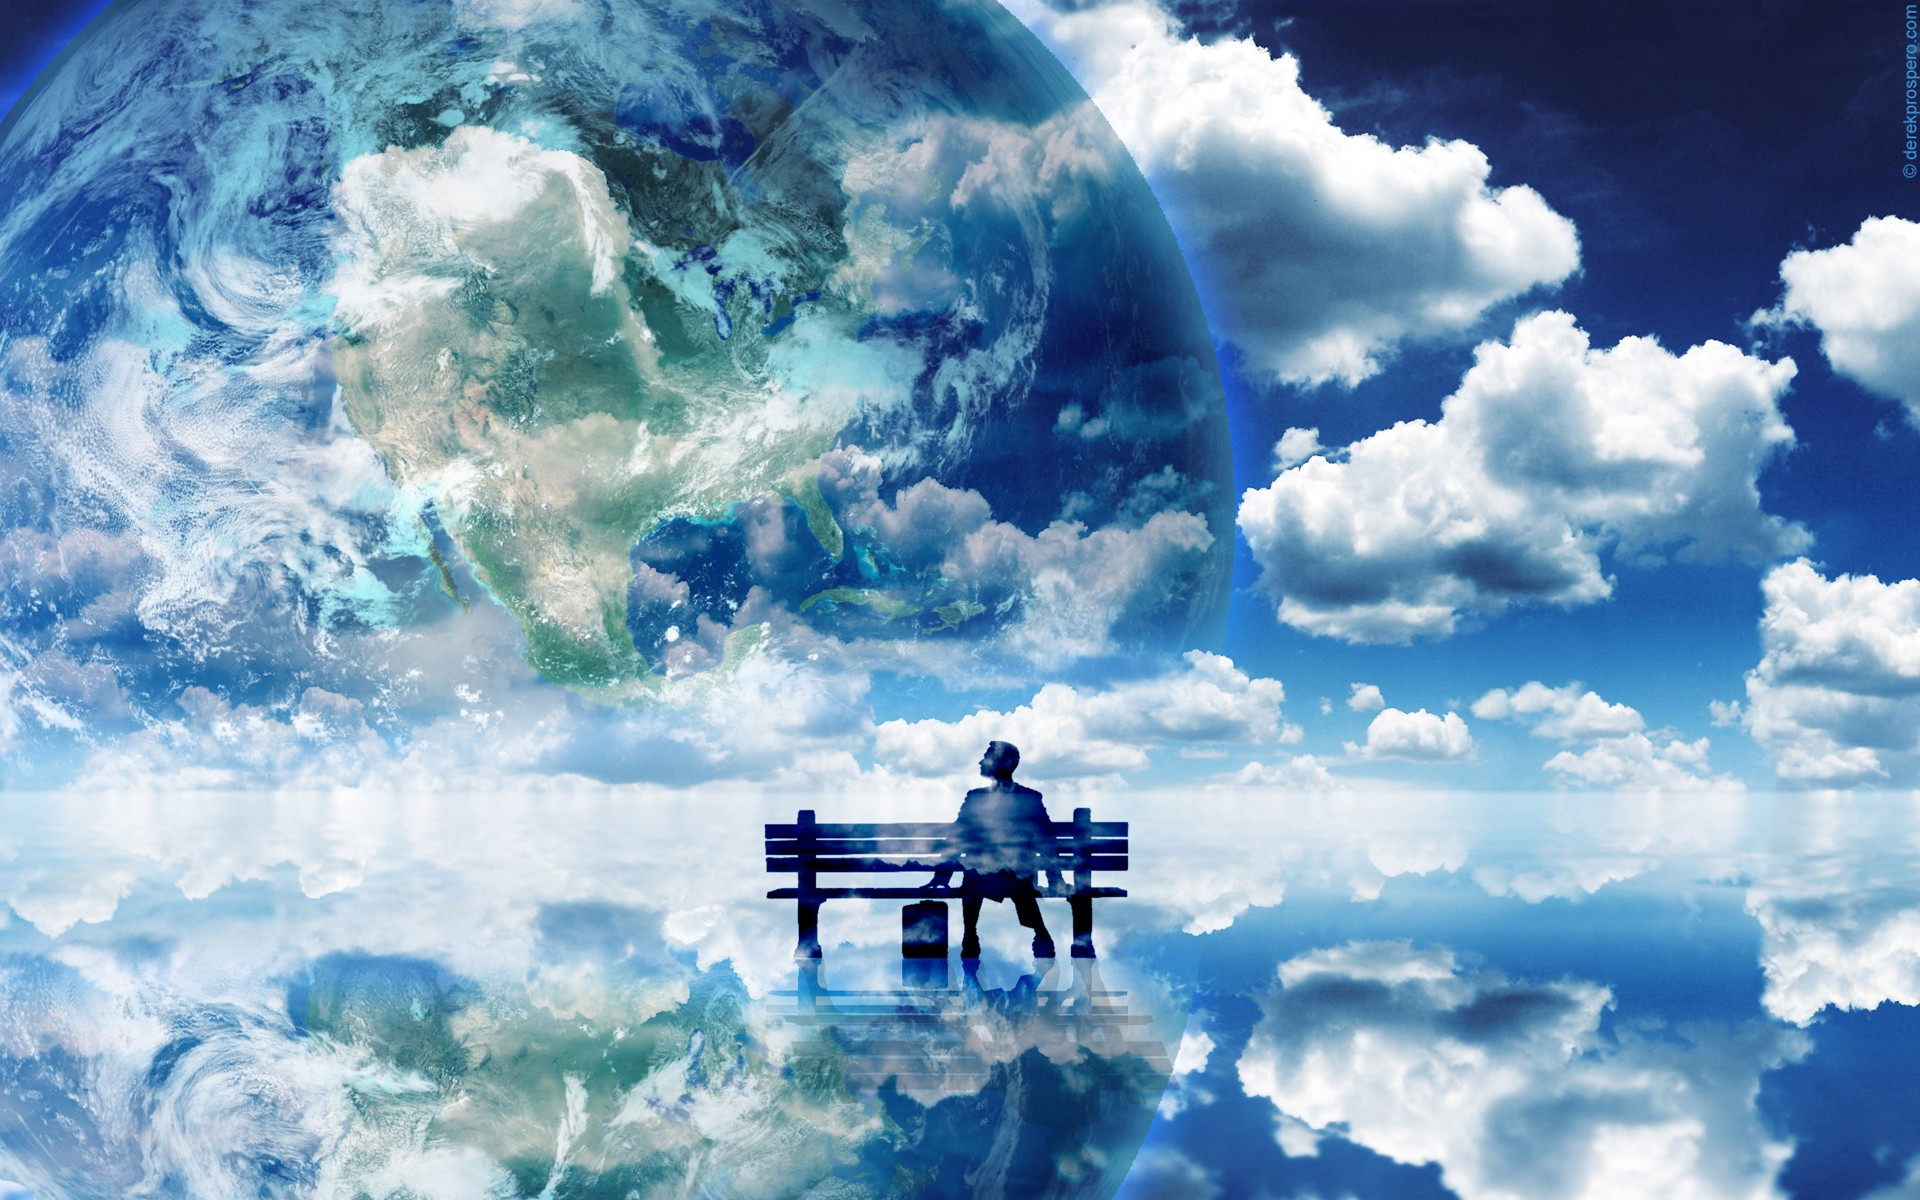
\includegraphics[width=\textwidth]{figures/eternityInHeart.jpg}

\note{09:48}
\note[item]{God has always made Himself known to man}
\note[item]{What does the passage mean? \emph{Man innately understands the possibility that something could exist beyond his own world.}}
\note[item]{However God may have chosen to speak to us, He was always going to leverage that part of our being that understands there's something more to life.}
\note[item]{Romans 1 -- Creation speaks to an `un-caused cause', which should lead us to consider God.}

\end{frame}

\begin{frame}
	\frametitle{In the past, God spoke to the Fathers by the prophets}
	\framesubtitle{Hebrews 1:1-2}
	\begin{center}
	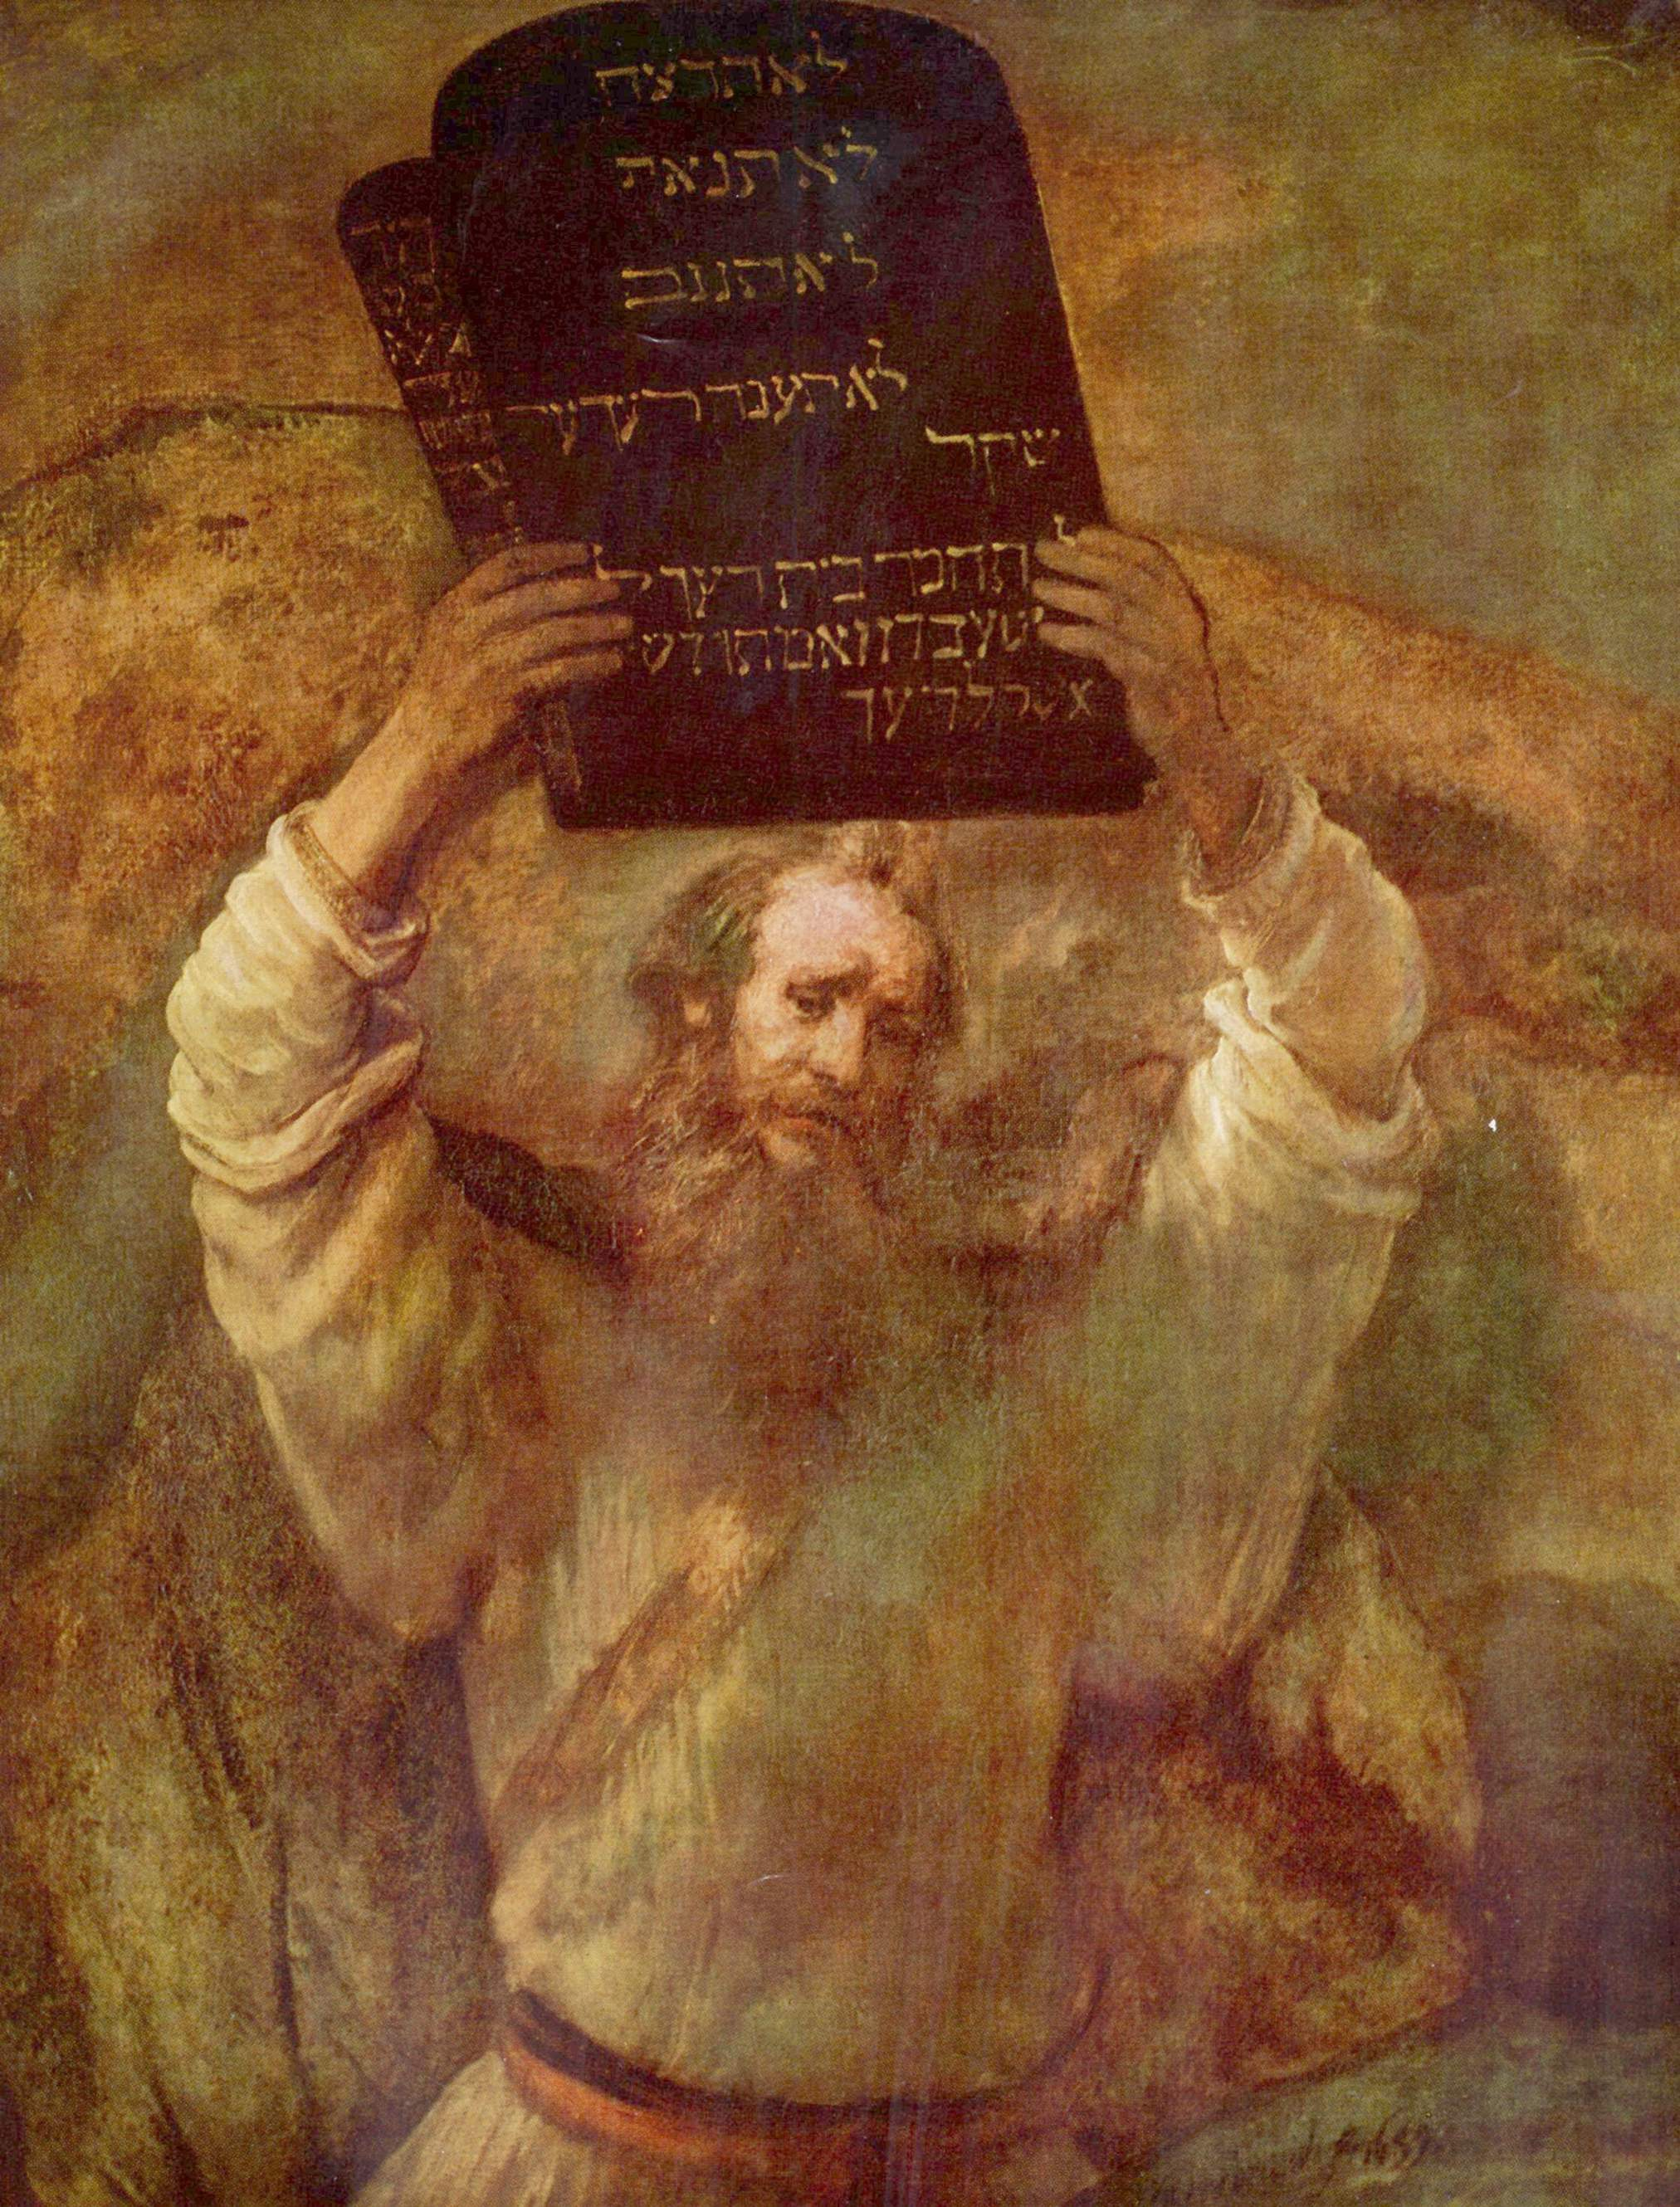
\includegraphics[height=0.8\textheight]{figures/mosesTenCommandments.jpg}
	\end{center}
	
	\note{09:50}
	\note[item]{The Israelites would have viewed Moses as the greatest prophet, the giver of God's Law.}
	\note[item]{Prophets would also include all those people we normally think of as prophets, whose main purpose was to plead for Israel to repent from wickedness.}
	\note[item]{The author leaves out the patriarchs. But, remember, he's just trying to make a point.}
	\note[item]{What's tough about learning from prophets? \emph{People don't have access to prophets all the time.  And, prophets just `tell' you what perfect faithfulness looks like.  They can't `show' you what perfect faithfulness looks like.}}
	\note[item]{Painting:Rembrandt}
\end{frame}

\begin{frame}
	\frametitle{Today, God speaks to us in His Son, Jesus}
	\framesubtitle{Hebrews 1:1-2}
	\begin{center}
	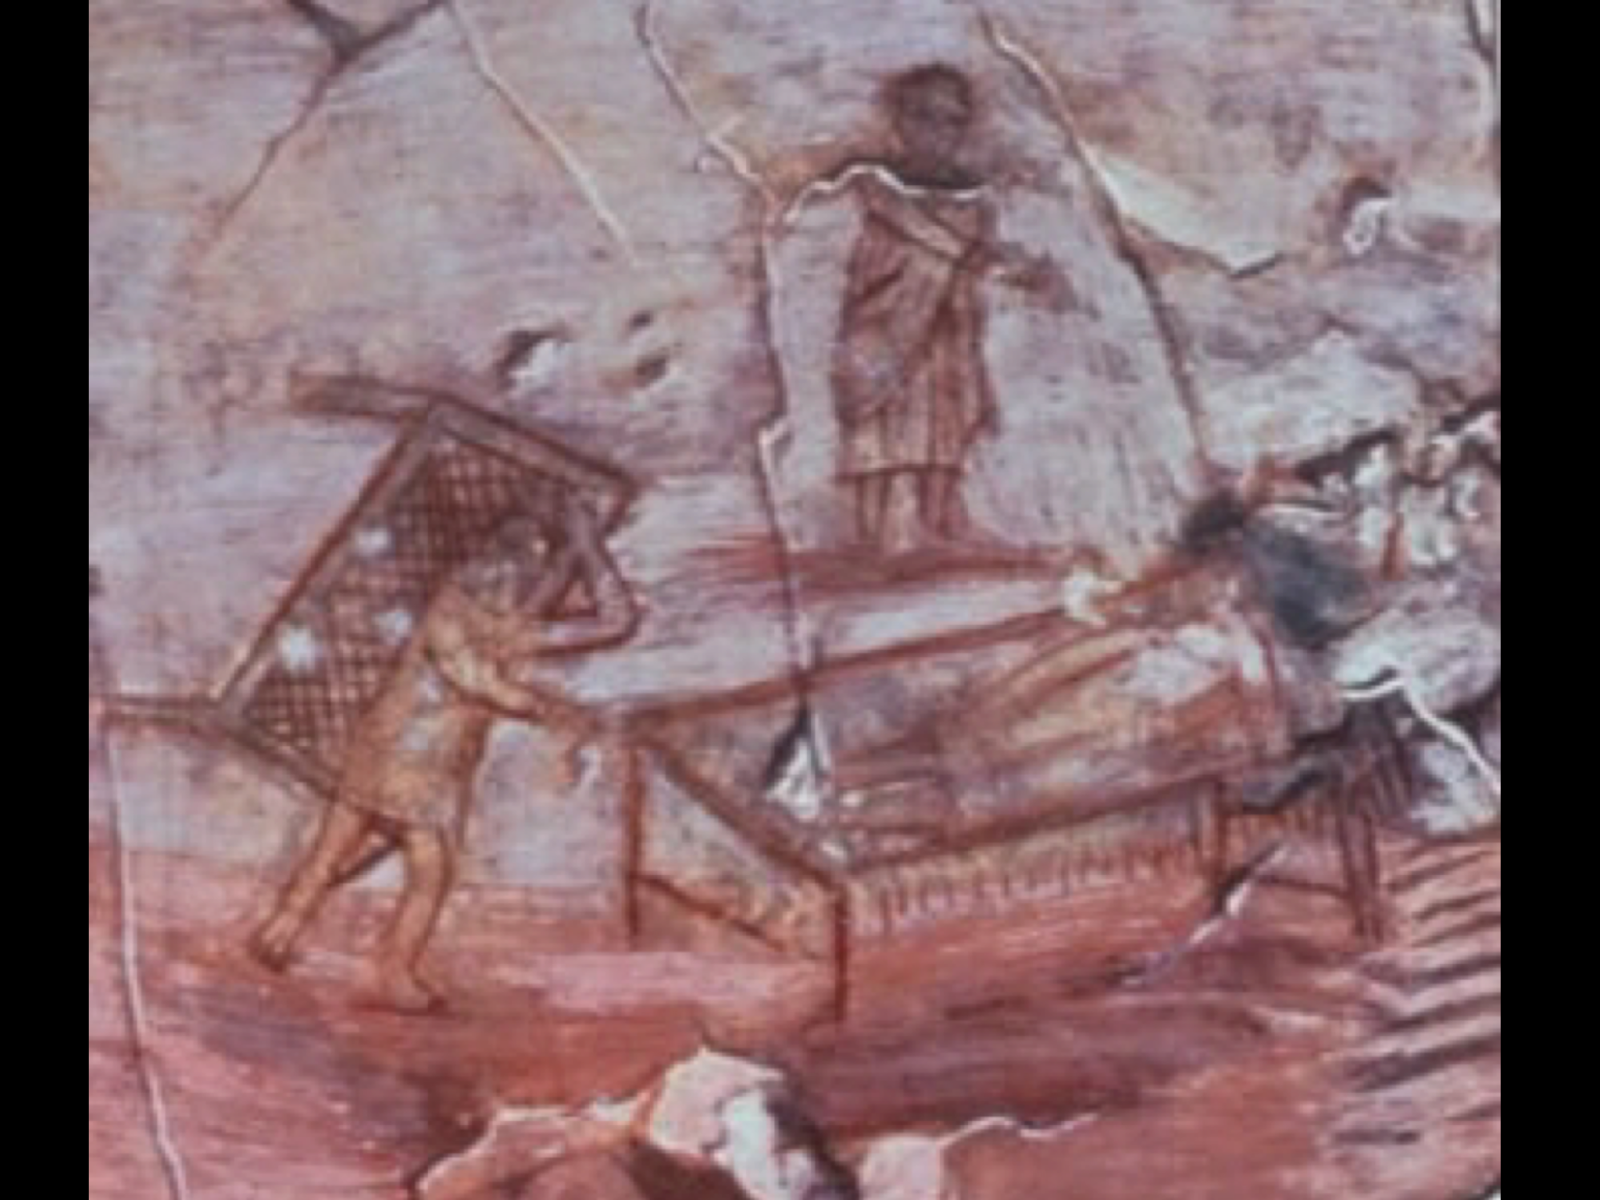
\includegraphics[height=0.8\textheight]{figures/jesusHealingParalytic.png}
	\end{center}
	
	\note{09:53}
	\note[item]{Speak means much more than simply teaching.}
	\note[item]{Jesus' life itself was God showing us how to live righteous.}
	\note[item]{God was under no obligation to do this.  He loved us.}
	\note[item]{But, even with Jesus, you only had direct access to his life if you lived in 1st century Palestine.}
	\note[item]{The fresco pictured is also from Dura-Europos (225AD), but a church instead of a synagogue.  It pictures Jesus healing the paralytic.  It's the earliest known depiction of Jesus.  In general, early Christians did not make images of Jesus.}
\end{frame}

\begin{frame}
	\frametitle{...And by extension His Word}
	\framesubtitle{Hebrews 1:1-2}
	\begin{center}
	
\includegraphics[width=\textheight]{figures/godSpeaksThroughTheWord.jpg}
	\end{center}
	
	\note{09:57}
	\note[item]{God has always shown Himself to man, but never more easily and more clearly than today}
	\note[item]{The Bible doesn't change through time.}
	\note[item]{The Bible is easily available for most people.}
	\note[item]{God makes himself `our God' when we read His word, understand it, and believe it}.
\end{frame}

\section{What does that mean for me?}

\begin{frame}
	\frametitle{God gives you moral anchor}
	\framesubtitle{Luke 4:1-13}
	\begin{columns}
	\begin{column}{0.5\textwidth}
	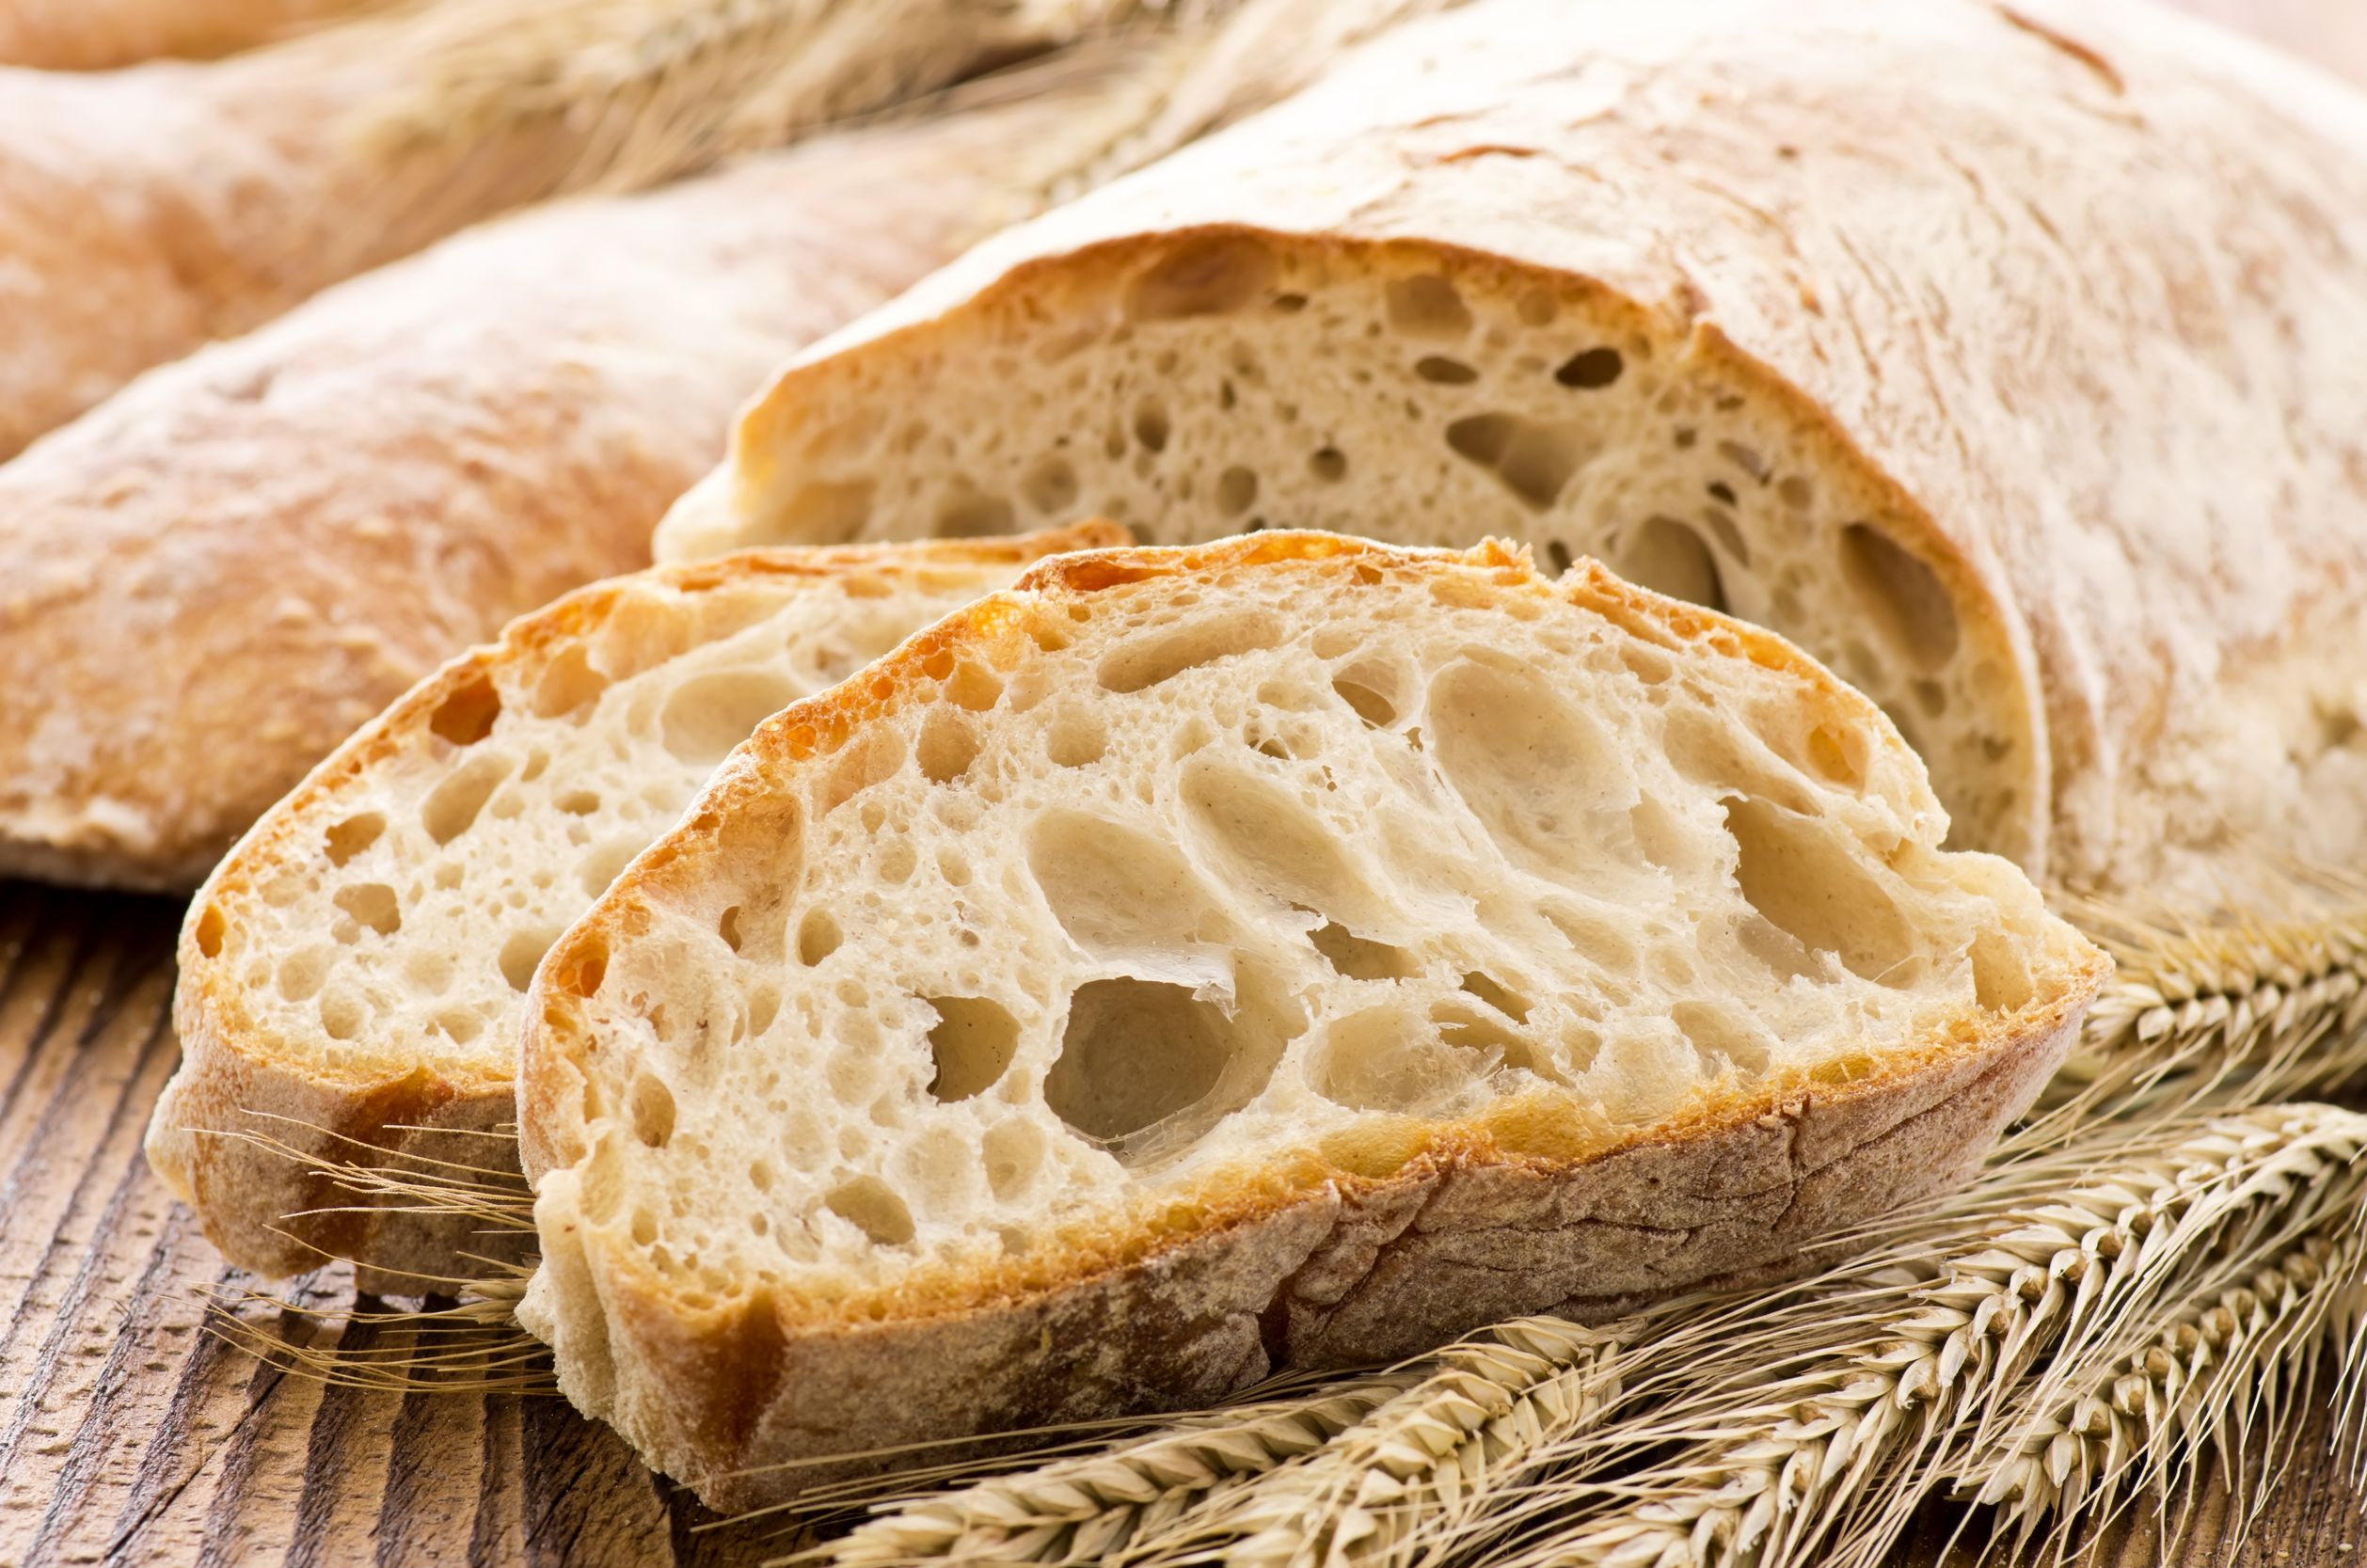
\includegraphics[width=\textwidth]{figures/bread.jpg}
	\end{column}
	\begin{column}{0.5\textwidth}
	\begin{itemize}
	\item Jesus used God as His basis for refuting Satan
	\item There is no objective morality without a God-provided standard
	\end{itemize}
	\end{column}
	\end{columns}
	
	\note{10:00}
	\note[item]{When God is `our' God, He sets the rules.}
	\note[item]{Jesus did not just quote any old verses from the Old Testament.}
	\note[item]{Every rebuttal was predicated on a respect for the greatness and authority of God.}
	\note[item]{Atheists, and indeed people in general, don't want an objective morality, until they become dissatisfied with their life}
	\note[item]{But, when we humble ourselves before God, we find refuge in the objective morality He provides.}
\end{frame}

\begin{frame}
	\frametitle{Love toward God is the foundation of eternal life}
	\framesubtitle{Luke 10:25-27}
	\begin{columns}
	\begin{column}{0.5\textwidth}
		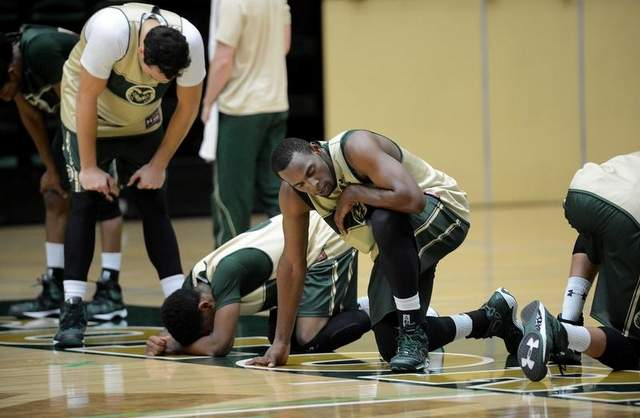
\includegraphics[width=\columnwidth]{figures/basketballRunning.jpg}
	\end{column}
	\begin{column}{0.5\textwidth}
		\begin{itemize}
			\item The main thing is to keep the main thing the main thing. -- {\footnotesize \emph{Steven Covey}}
			\item Sometimes we don't remember what giving all of ourselves looks like.
		\end{itemize}
	\end{column}
	\end{columns}
	\note{10:05}
	\note[item]{Loving God with all of ourselves is a `must have' for salvation.}
	\note[item]{We are not perfect.}
	\note[item]{In spite of that, though, we have to keep pushing.}
	\note[item]{Remember that we haven't given everything, yet.  We can always push to love God more.}
\end{frame}

\section{Review}

\begin{frame}
\frametitle{I will be their God}
\framesubtitle{God wants to be \emph{your} God}
\begin{columns}[c]
\begin{column}{0.3\textwidth}
	
\includegraphics[width=\columnwidth]{figures/uncleSam.jpg}
\end{column}
\begin{column}{0.7\textwidth}
	\begin{itemize}
		\item God is great and mighty
		\item God loves and blesses us.
		\item God shows Himself to man
		\item God's portrait is perfected in Jesus
		\item We meet Jesus in the Bible.  
		\item Respect for God can guide our lives
		\item Loving God is where salvation starts
	\end{itemize}
\end{column}
\end{columns}
\note{10:10}
\note[item]{Are you proud of being on God's team?}
\end{frame}

\chapter{They Shall be My People}

\begin{goals}
\goal God wants people who choose Him voluntarily.
\goal Understand the different ways God uses to call us to Him.
\goal Appreciate how unique and special a Christians' relationship with God is.
\end{goals}

\intro

\lipsum[4]

\bible

\begin{quote}
\lipsum[4] \bv{Jeremiah}{(31:31-33)}
\end{quote}

\begin{quote}
\lipsum[4] \bv{Jeremiah}{(31:31-33)}
\end{quote}

\begin{quote}
\lipsum[4] \bv{Jeremiah}{(31:31-33)}
\end{quote}

\begin{quote}
\lipsum[4] \bv{Jeremiah}{(31:31-33)}
\end{quote}

\discussion

\lipsum[5-7]

\questions

Question 1: Knowledge
\vfill

Question 2: Comprehension
\vfill

Question 3: Application
\vfill

Question 4: Analysis
\vfill

Question 5: Synthesis
\vfill

Question 6: Evaluation
\vfill

\chapter{For They Shall All Know Me}

\begin{goals}
\goal Show that God's people are now joined by a common faith not a common ancestry 
\goal Elaborate on what it means to `know' God
\goal Come up with a plan to know God better
\end{goals}

\begin{bible}
\bve{Romans}{(4:1-25)}
What then shall we say was gained by Abraham, our forefather according to the flesh? 2 For if Abraham was justified by works, he has something to boast about, but not before God. 3 For what does the Scripture say? ``Abraham believed God, and it was counted to him as righteousness.'' 4 Now to the one who works, his wages are not counted as a gift but as his due. 5 And to the one who does not work but believes in him who justifies the ungodly, his faith is counted as righteousness, 6 just as David also speaks of the blessing of the one to whom God counts righteousness apart from works:
\begin{quote}
7 ``Blessed are those whose lawless deeds are forgiven, and whose sins are covered;
8 blessed is the man against whom the Lord will not count his sin.''
\end{quote}
9 Is this blessing then only for the circumcised, or also for the uncircumcised? For we say that faith was counted to Abraham as righteousness. 10 How then was it counted to him? Was it before or after he had been circumcised? It was not after, but before he was circumcised. 11 He received the sign of circumcision as a seal of the righteousness that he had by faith while he was still uncircumcised. The purpose was to make him the father of all who believe without being circumcised, so that righteousness would be counted to them as well, 12 and to make him the father of the circumcised who are not merely circumcised but who also walk in the footsteps of the faith that our father Abraham had before he was circumcised.

13 For the promise to Abraham and his offspring that he would be heir of the world did not come through the law but through the righteousness of faith. 14 For if it is the adherents of the law who are to be the heirs, faith is null and the promise is void. 15 For the law brings wrath, but where there is no law there is no transgression.

16 That is why it depends on faith, in order that the promise may rest on grace and be guaranteed to all his offspring--not only to the adherent of the law but also to the one who shares the faith of Abraham, who is the father of us all, 17 as it is written, ``I have made you the father of many nations''--in the presence of the God in whom he believed, who gives life to the dead and calls into existence the things that do not exist. 18 In hope he believed against hope, that he should become the father of many nations, as he had been told, ``So shall your offspring be.'' 19 He did not weaken in faith when he considered his own body, which was as good as dead (since he was about a hundred years old), or when he considered the barrenness of Sarah's womb. 20 No unbelief made him waver concerning the promise of God, but he grew strong in his faith as he gave glory to God, 21 fully convinced that God was able to do what he had promised. 22 That is why his faith was ``counted to him as righteousness.'' 23 But the words ``it was counted to him'' were not written for his sake alone, 24 but for ours also. It will be counted to us who believe in him who raised from the dead Jesus our Lord, 25 who was delivered up for our trespasses and raised for our justification.

\bvh{Philippians}{(3:3-10)}
1 For we are the circumcision, the ones who serve by the Spirit of God, boast in Christ Jesus, and do not put confidence in the flesh-- 4 although I once also had confidence in the flesh. If anyone else thinks he has grounds for confidence in the flesh, I have more: 5 circumcised the eighth day; of the nation of Israel, of the tribe of Benjamin, a Hebrew born of Hebrews; regarding the law, a Pharisee; 6 regarding zeal, persecuting the church; regarding the righteousness that is in the law, blameless.

7 But everything that was a gain to me, I have considered to be a loss because of Christ. 8 More than that, I also consider everything to be a loss in view of the surpassing value of knowing Christ Jesus my Lord. Because of Him I have suffered the loss of all things and consider them filth, so that I may gain Christ 9 and be found in Him, not having a righteousness of my own from the law, but one that is through faith in Christ--the righteousness from God based on faith. 10 My goal is to know Him and the power of His resurrection and the fellowship of His sufferings, being conformed to His death,

\bve{Ephesians}{(3:14-18)}
14 For this reason I bow my knees before the Father, 15 from whom every family in heaven and on earth is named, 16 that according to the riches of his glory he may grant you to be strengthened with power through his Spirit in your inner being, 17 so that Christ may dwell in your hearts through faith--that you, being rooted and grounded in love, 18 may have strength to comprehend with all the saints what is the breadth and length and height and depth,

\bvh{Matthew}{(7:7-12)}
7 ``Keep asking, and it will be given to you. Keep searching, and you will find. Keep knocking, and the door will be opened to you. 8 For everyone who asks receives, and the one who searches finds, and to the one who knocks, the door will be opened. 9 What man among you, if his son asks him for bread, will give him a stone? 10 Or if he asks for a fish, will give him a snake? 11 If you then, who are evil, know how to give good gifts to your children, how much more will your Father in heaven give good things to those who ask Him! 12 Therefore, whatever you want others to do for you, do also the same for them--this is the Law and the Prophets.

\end{bible}

\begin{discussion}
\dsubsec{Introduction}{900-905}{5}

\dsubsec{Show that God's people are now joined by a common faith not a common ancestry }{905-915}{10}

\bvs{Romans}{(4:1-25)} Those who have the faith of Abraham are his children.

\bvs{Phil}{(3:3-10)} Lesson 9. also says we are the true circumcision.

\dsubsec{Elaborate on what it means to `know' God}{915-925}{10}

These passages emphasize the importance of knowing God, but not necessarily what there is to know!.
\bvs{Ephesians}{(3:14-18)} Lesson 9

\dsubsec{Come up with a plan to know God better}{925-940}{15}

\bvs{Matthew}{(7:7-12)} Keep asking and it will be given you.

\dsubsec{Review}{940-945}{5}
\end{discussion}

\begin{questions}
\q Thinking about Romans 4, interpret the phrase ``For they shall \emph{all} know me'' from Jeremiah 31:34
\q Explain the weakness of God's special people being based on physical genealogy under the Old Covenant.
\q Given that Christians are now God's special people, what should we focus on according to Philippians 3:3-10 and Ephesians 3:14-18.
\q List four practical you could try to know God better.
\end{questions}

\end{document}


